\documentclass[border=2pt]{standalone}
\usepackage{fontspec}
\usepackage{unicode-math}
\setmainfont{Libertinus Serif}
\setsansfont{Libertinus Sans}
\setmathfont{Libertinus Math}[Scale=MatchUppercase]
\setmonofont{JetBrainsMono-Regular.ttf}[Path=../fonts/,ItalicFont=JetBrainsMono-Italic.ttf,Scale=0.95,RawFeature={-liga,-calt,-clig,-dlig}]
\usepackage{amsmath}
\providecommand{\llbracket}{[\![}
\providecommand{\rrbracket}{]\!]}
\usepackage{tikz}
\usetikzlibrary{positioning,arrows.meta,fit,backgrounds,calc,decorations.pathreplacing,decorations.markings,shapes.misc,matrix,shadings}

\definecolor{ink}{HTML}{1F2328}
\definecolor{muted}{HTML}{5B6470}
\definecolor{hairline}{HTML}{C9CFD6}
\definecolor{paper}{HTML}{FFFFFF}
\definecolor{pass}{HTML}{007A59}   \definecolor{passsoft}{HTML}{DAF1E9}
\definecolor{back}{HTML}{7A3E65}   \definecolor{backsoft}{HTML}{F1E1EB}
\definecolor{backdeep}{HTML}{70355C}
\definecolor{keep}{HTML}{006A91}   \definecolor{keepsoft}{HTML}{DCE9F5}
\definecolor{meas}{HTML}{9A5B00}   \definecolor{meassoft}{HTML}{FBEFD5}
\definecolor{measdeep}{HTML}{885000}
\definecolor{bad}{HTML}{AF4900}    \definecolor{badsoft}{HTML}{F9E1D3}
\definecolor{light}{HTML}{167BB4}  \definecolor{lightsoft}{HTML}{E3F2FB}

\tikzset{
  house/.style={>={Stealth[length=1.35mm, width=.95mm]}, line width=0.6pt,
    every node/.style={font=\small, text=ink}},
  flowmark/.style={postaction={decorate},decoration={markings,
    mark=at position .60 with {\arrow{Stealth[length=1.15mm,width=.8mm]}}}},
  box/.style={draw=ink, line width=0.6pt, rounded corners=1.8pt, inner xsep=5pt, inner ysep=3.5pt,
    align=center, fill=paper},
  boxdim/.style={box, draw=hairline, text=muted},
  boxpass/.style={box, draw=pass, shade,left color=passsoft!45!white,right color=passsoft},
  boxback/.style={box, draw=back, shade,left color=backsoft!45!white,right color=backsoft},
  boxkeep/.style={box, draw=keep, shade,left color=keepsoft!45!white,right color=keepsoft},
  boxmeas/.style={box, draw=meas, shade,left color=meassoft!45!white,right color=meassoft},
  boxbad/.style={box, draw=bad, shade,left color=badsoft!45!white,right color=badsoft},
  body/.style={box, shade,top color=white,bottom color=ink!5!white,
    minimum width=10mm, minimum height=11mm, font=\normalsize},
  wire/.style={draw=ink, line width=0.8pt},
  wpass/.style={draw=pass, line width=0.9pt},
  wback/.style={draw=back, line width=0.9pt},
  wkeep/.style={draw=keep, line width=0.9pt},
  wmeas/.style={draw=meas, line width=0.9pt},
  cwire/.style={draw=ink, line width=0.4pt, double, double distance=1.1pt},
  cmeas/.style={draw=meas, line width=0.45pt, double, double distance=1.1pt},
  flow/.style={->, draw=ink, line width=0.6pt},
  flowdim/.style={->, draw=muted, line width=0.5pt},
  lab/.style={font=\footnotesize, text=ink, inner sep=1.5pt},
  labpass/.style={lab, text=pass!80!black},
  labback/.style={lab, text=backdeep},
  labkeep/.style={lab, text=keep},
  labmeas/.style={lab, text=measdeep},
  labbad/.style={lab, text=bad},
  note/.style={font=\footnotesize, text=muted, align=left, inner sep=1.5pt},
  head/.style={font=\small\bfseries, text=ink, inner sep=1.5pt},
  panel/.style={font=\footnotesize\itshape, text=muted, inner sep=1.5pt},
  group/.style={draw=hairline, dashed, rounded corners=2.5pt, inner sep=5pt},
  gate/.style={draw=ink, fill=paper, line width=0.6pt, rounded corners=1.2pt, minimum size=6mm, inner sep=2pt},
  ctrl/.style={circle, fill=ink, inner sep=0pt, minimum size=1.6mm},
  octrl/.style={circle, draw=ink, fill=paper, inner sep=0pt, minimum size=1.6mm, line width=0.6pt},
  dot/.style={circle, fill=ink, inner sep=0pt, minimum size=1.5mm},
  meter/.style={draw=meas, fill=meassoft, line width=0.6pt, rounded corners=1.2pt, minimum width=7mm,
    minimum height=5.6mm, inner sep=0pt,
    path picture={\draw[measdeep, line width=0.5pt] ($(path picture bounding box.center)+(-2mm,-1.2mm)$) arc (180:0:2mm);
                  \draw[measdeep, line width=0.5pt, ->] ($(path picture bounding box.center)+(0,-1.2mm)$) -- ++(1.4mm,2.1mm);}},
  cell/.style={draw=hairline, minimum width=7mm, minimum height=5.5mm, inner sep=0pt, font=\footnotesize},
}
\newcommand{\feedbackcurve}[3]{\draw[wback, postaction={decorate}, decoration={markings, mark=at position .5 with {\arrow{Stealth[length=1.3mm,width=.9mm]}}}]
    ($(#1.east)+(0,-2.6mm)$) -- ($(#1.east)+({max(#3-0.55,0.15)},-2.6mm)$)
    to[out=0,in=0,looseness=1.7] ($(#1.east)+({max(#3-0.55,0.15)},-2.6mm)+(0,-#2)$)
    -- ($(#1.west)+({-max(#3-0.55,0.15)},-2.6mm)+(0,-#2)$)
    to[out=180,in=180,looseness=1.7] ($(#1.west)+({-max(#3-0.55,0.15)},-2.6mm)$)
    -- ($(#1.west)+(0,-2.6mm)$);}
\newcommand{\feedbackcurvez}[4]{\draw[wback]
    ($(#1.east)+(0,-2.6mm)$) -- ($(#1.east)+({max(#3-0.55,0.15)},-2.6mm)$)
    to[out=0,in=0,looseness=1.7] ($(#1.east)+({max(#3-0.55,0.15)},-2.6mm)+(0,-#2)$)
    -- node[boxback, font=\footnotesize, inner xsep=3pt, inner ysep=2pt] {#4}
       ($(#1.west)+({-max(#3-0.55,0.15)},-2.6mm)+(0,-#2)$)
    to[out=180,in=180,looseness=1.7] ($(#1.west)+({-max(#3-0.55,0.15)},-2.6mm)$)
    -- ($(#1.west)+(0,-2.6mm)$);
  \draw[wback,-{Stealth[length=1.3mm,width=.9mm]}] ($(#1.west)+(-0.12,-2.6mm)+(0,-#2)$) -- ++(-0.01,0);}
\newcommand{\feedbackcurveat}[4]{\draw[wback, postaction={decorate}, decoration={markings, mark=at position .5 with {\arrow{Stealth[length=1.3mm,width=.9mm]}}}]
    ($(#1.east)+(0,-#2)$) -- ($(#1.east)+({max(#4-0.55,0.15)},-#2)$)
    to[out=0,in=0,looseness=1.7] ($(#1.east)+({max(#4-0.55,0.15)},-#2)+(0,-#3)$)
    -- ($(#1.west)+({-max(#4-0.55,0.15)},-#2)+(0,-#3)$)
    to[out=180,in=180,looseness=1.7] ($(#1.west)+({-max(#4-0.55,0.15)},-#2)$)
    -- ($(#1.west)+(0,-#2)$);}
\newcommand{\backloop}[3]{\draw[wback, rounded corners=3pt] ($(#1.east)+(0,-2.6mm)$) -- ++(#3,0) -- ++(0,-#2) -- ($(#1.west)+(-#3,-2.6mm)+(0,-#2)$) -- ($(#1.west)+(-#3,-2.6mm)$) -- ($(#1.west)+(0,-2.6mm)$);}
\newcommand{\ket}[1]{\lvert #1\rangle}
\newcommand{\bra}[1]{\langle #1\rvert}
\newcommand{\kw}[1]{\texttt{#1}}
\providecommand{\Tr}{\operatorname{Tr}}
\hyphenpenalty=10000 \exhyphenpenalty=10000

\begin{document}
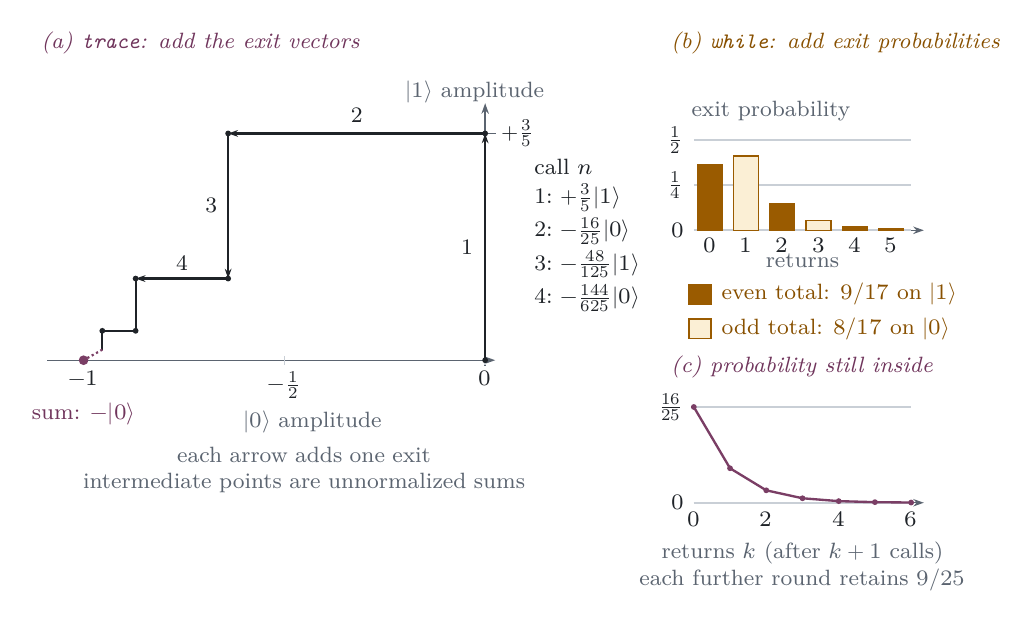
\begin{tikzpicture}[house]
\node[panel,anchor=west,text=backdeep] at (0,4.03) {(a) \texttt{trace}: add the exit vectors};
\node[panel,anchor=west,text=measdeep] at (8.0,4.03) {(b) \texttt{while}: add exit probabilities};
\begin{scope}[xshift=5.7cm,x=5.1cm,y=4.8cm]
 \draw[flowdim] (-1.09,0)--(.025,0);
 \draw[flowdim] (0,-.015)--(0,.68);
 \draw[muted,line width=.45pt] (0,.60)--(.027,.60);
 \node[lab,anchor=west] at (.028,.60) {$+\tfrac35$};
 \node[note,anchor=west] at (-.21,.71) {$\ket1$ amplitude};
 \foreach \xx/\txt in {-1/{-1},-.5/{-\frac12},0/0}{
  \draw[hairline] (\xx,-.012)--(\xx,.012);
  \node[lab,anchor=north] at (\xx,-.016) {$\txt$};}

 \tikzset{walkstep/.style={draw=ink,line width=.8pt,-{Stealth[length=1.25mm,width=.85mm]}}}
 \draw[walkstep] (0,0)--(0,.6);
 \draw[walkstep] (0,.6)--(-.64,.6);
 \draw[walkstep] (-.64,.6)--(-.64,.216);
 \draw[walkstep] (-.64,.216)--(-.8704,.216);
 \draw[ink,line width=.7pt] (-.8704,.216)--(-.8704,.07776)
  --(-.953344,.07776)--(-.953344,.0279936);
 \draw[back,densely dotted,line width=.8pt] (-.953344,.0279936)--(-1,0);
 \foreach \p in {(0,0),(0,.6),(-.64,.6),(-.64,.216),(-.8704,.216),(-.8704,.07776),(-.953344,.07776)}
  \fill[ink] \p circle (1.05pt);
 \fill[back] (-1,0) circle (1.75pt);
 \node[lab,anchor=east] at (-.018,.3) {1};
 \node[lab,anchor=south] at (-.32,.615) {2};
 \node[lab,anchor=east] at (-.655,.41) {3};
 \node[lab,anchor=south] at (-.755,.225) {4};
 \node[lab,anchor=west,align=left] at (.11,.33)
  {call $n$\\[1pt] 1:\ $+\tfrac35\ket1$\\[1pt] 2:\ $-\tfrac{16}{25}\ket0$\\[1pt] 3:\ $-\tfrac{48}{125}\ket1$\\[1pt] 4:\ $-\tfrac{144}{625}\ket0$};
 \node[labback,anchor=north,align=center] at (-1,-.10) {sum: $-\ket0$};
 \node[note,anchor=north] at (-.43,-.12) {$\ket0$ amplitude};
\end{scope}
\node[note,anchor=north,align=center,text width=67mm] at (3.4,-1.04)
 {each arrow adds one exit\\intermediate points are unnormalized sums};
\begin{scope}[xshift=8.35cm,yshift=1.65cm,x=.46cm,y=2.3cm,
 even bar/.style={fill=meas,draw=meas,line width=.55pt},
 odd bar/.style={fill=meassoft,draw=meas,line width=.55pt}]
 \draw[flowdim] (0,0)--(6.35,0);
 \foreach \yy/\txt in {0/0,.25/{\frac14},.5/{\frac12}}{
  \draw[hairline] (0,\yy)--(6,\yy);
  \node[lab,anchor=east] at (-.14,\yy) {$\txt$};}
 \node[note,anchor=west] at (-.2,.66) {exit probability};
 \foreach \ii/\pp/\toOne in
  {0/.36/1,1/.4096/0,2/.147456/1,3/.05308416/0,4/.0191102976/1,5/.006879707136/0}{
  \ifnum\toOne=1
   \path[even bar] (\ii+.10,0) rectangle (\ii+.78,\pp);
  \else
   \path[odd bar] (\ii+.10,0) rectangle (\ii+.78,\pp);
  \fi
  \node[lab,anchor=north] at (\ii+.44,-.012) {$\ii$};
 }
 \node[note,anchor=north] at (3,-.105) {returns};
 \node[labmeas,anchor=north west] (even) at (.63,-.265) {even total: $9/17$ on $\ket1$};
 \path[even bar] ([xshift=-3.5mm,yshift=-1.25mm]even.west)
   rectangle ([xshift=-.7mm,yshift=1.25mm]even.west);
 \node[labmeas,anchor=north west] (odd) at (.63,-.455) {odd total: $8/17$ on $\ket0$};
 \path[odd bar] ([xshift=-3.5mm,yshift=-1.25mm]odd.west)
   rectangle ([xshift=-.7mm,yshift=1.25mm]odd.west);
\end{scope}

\node[panel,anchor=west,text=backdeep] at (8.0,-.09) {(c) probability still inside};
\begin{scope}[xshift=8.35cm,yshift=-1.81cm,x=.46cm,y=1.9cm]
 \draw[flowdim] (0,0)--(6.35,0);
 \foreach \yy/\txt in {0/0,.64/{\frac{16}{25}}}{
  \draw[hairline] (0,\yy)--(6,\yy);
  \node[lab,anchor=east] at (-.14,\yy) {$\txt$};}
 \foreach \xx in {0,2,4,6}
  \node[lab,anchor=north] at (\xx,-.025) {$\xx$};
 \draw[back,line width=.85pt] plot coordinates
 {(0,.64)(1,.2304)(2,.082944)(3,.02985984)
  (4,.0107495424)(5,.003869835264)(6,.00139314069504)};
 \foreach \xx/\yy in {0/.64,1/.2304,2/.082944,3/.02985984,
  4/.0107495424,5/.003869835264,6/.00139314069504}
  \fill[back] (\xx,\yy) circle (1.05pt);
 \node[note,anchor=north,align=center] at (3,-.23)
  {returns $k$ (after $k+1$ calls)\\each further round retains $9/25$};
\end{scope}
\end{tikzpicture}
\end{document}
